\documentclass[lettersize,journal]{IEEEtran}
\usepackage{amsmath,amsfonts,amssymb}
\usepackage{algorithmic}
\usepackage{algorithm}
\usepackage{array}
\usepackage[caption=false,font=normalsize,labelfont=sf,textfont=sf]{subfig}
\usepackage{textcomp}
\usepackage{stfloats}
\usepackage{url}
\usepackage{verbatim}
\usepackage{graphicx}
\usepackage{cite}
\usepackage{booktabs}
\usepackage{multirow}
\usepackage{tikz}
\usepackage[colorlinks,linkcolor=red,anchorcolor=blue,citecolor=green]{hyperref}
\usetikzlibrary{arrows.meta,positioning,fit,backgrounds,calc,shadows}
\hyphenation{op-tical net-works semi-conduc-tor IEEE-Xplore}

\begin{document}

\title{PhyST-Net: An Exogenous-Aware Spatio-Temporal Graph Transformer for Domain-Constrained Network Forecasting}

\author{Xu~Li
\thanks{Xu Li is with Tongji University, Shanghai, China (e-mail: 2534163@tongji.edu.cn).}%
}

\markboth{{\it Paper}}%
{X.~Li: PhyST-Net for Domain-Constrained Network Forecasting}

\maketitle

\begin{abstract}
Spatio-temporal forecasting is a core task for graph-structured networks such as power grids, traffic systems, and industrial sensor clusters, where accurate node-level prediction requires joint modeling of historical trends, external drivers, and operational constraints. Existing forecasting models often treat historical covariates, future exogenous variables, and domain priors as isolated inputs, limiting their ability to capture the interplay between temporal continuity, dynamic spatial topology, and physical feasibility. This paper proposes PhyST-Net, an exogenous-aware spatio-temporal graph Transformer designed as a general framework for domain-constrained network forecasting. PhyST-Net formulates prediction as a multi-modal graph learning task with historical target states, historical exogenous variables (ExG), future ExG, and graph metadata as distinct interfaces. The framework employs: (1) Adaptive Gaussian-soft-windowed Patching (AGSP) for continuous temporal tokenization; (2) a Relational Spatio-Temporal Manifold Fusion (R-STMF) graph adapter for multi-scale spatial dependency modeling; (3) KAN-enhanced Adaptive Conditioning (K-AC) for non-linear exogenous modulation; and (4) a Domain-Informed Dynamic Capping Head (DI-DCH) for constraint-aware decoding. While the framework is general, we validate its effectiveness on the challenging task of wind power forecasting using the SDWPF, HoT, and Kelmarsh datasets. Results show that PhyST-Net consistently improves forecasting accuracy and feasibility across multiple horizons, demonstrating the value of explicit exogenous awareness and domain-informed architectural inductive biases.
\end{abstract}

\begin{IEEEkeywords}
Spatio-temporal forecasting, graph Transformers, exogenous variables, domain-constrained machine learning, network forecasting.
\end{IEEEkeywords}

\section{Introduction}
\label{sec:intro}
\IEEEPARstart{S}{patio-temporal} forecasting predicts future states in graph-structured systems (e.g., transportation networks, power grids) where temporal dynamics and spatial interactions evolve jointly. Node-level trajectories are rarely self-driven; rather, they are shaped by historical conditions, future external drivers, and domain-specific feasibility constraints. As illustrated in Fig.~\ref{fig:multi_scale_processes}, complex network signals comprise shared macro-trends driven by exogenous forcing and high-frequency local variations. Consequently, a practical forecasting model must learn continuous temporal representations, infer dynamic graph relations, and integrate future exogenous variables (ExG) without data leakage, all while maintaining operational compatibility.

\begin{figure}[htbp]
\centering
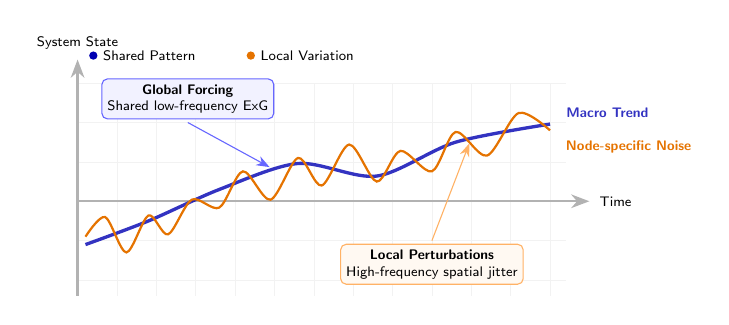
\begin{tikzpicture}[font=\sffamily\tiny, >=Stealth]
    % Coordinates and grid
    \draw[help lines, gray!10, step=0.5] (0,-1.2) grid (6.2,1.5);
    \draw[->, thick, gray!60] (0,0) -- (6.5,0) node[right, black] {Time};
    \draw[->, thick, gray!60] (0,-1.2) -- (0,1.8) node[above, black] {System State};
    
    % Macro trend (Blue)
    \draw[very thick, blue!70!black, smooth, opacity=0.8] 
        plot coordinates {(0.1,-0.55) (0.9,-0.25) (1.8,0.15) (2.8,0.48) (3.8,0.32) (4.8,0.75) (6.0,0.98)}
        node[right=2pt, yshift=4pt, font=\sffamily\tiny\bfseries, blue!70!black] {Macro Trend};
    
    % Local variation (Orange)
    \draw[thick, orange!90!black, smooth] 
        plot coordinates {(0.1,-0.45) (0.35,-0.2) (0.62,-0.65) (0.9,-0.18) (1.15,-0.42) (1.45,0.02) (1.8,-0.08) (2.1,0.38) (2.45,0.02) (2.8,0.55) (3.1,0.2) (3.45,0.72) (3.8,0.25) (4.1,0.64) (4.5,0.38) (4.8,0.88) (5.2,0.58) (5.6,1.12) (6.0,0.9)}
        node[right=2pt, yshift=-6pt, font=\sffamily\tiny\bfseries, orange!90!black] {Node-specific Noise};

    % Callouts
    \node[draw=blue!60, fill=blue!5, rounded corners=2pt, align=center, inner sep=2pt] at (1.4,1.3) 
        {\textbf{Global Forcing}\\Shared low-frequency ExG};
    \draw[->, blue!60, shorten >=2pt] (1.4,1.0) -- (2.5,0.4);

    \node[draw=orange!60, fill=orange!5, rounded corners=2pt, align=center, inner sep=2pt] at (4.5,-0.8) 
        {\textbf{Local Perturbations}\\High-frequency spatial jitter};
    \draw[->, orange!60, shorten >=2pt] (4.5,-0.5) -- (5.0,0.8);

    % Legend-like markers (Moved higher to avoid callout)
    \fill[blue!70!black] (0.2,1.85) circle (1.5pt) node[right, black] {Shared Pattern};
    \fill[orange!90!black] (2.2,1.85) circle (1.5pt) node[right, black] {Local Variation};

\end{tikzpicture}
\caption{Multi-scale spatio-temporal processes. General network signals are composed of shared macro-trends driven by exogenous forcing and high-frequency variations unique to individual nodes. PhyST-Net separates these components through dual-branch graph reasoning.}
\label{fig:multi_scale_processes}
\end{figure}

\subsection{The Forecasting Trilemma in Spatio-Temporal Networks}
\label{sec:trilemma}
Despite recent architectural advancements, modern spatio-temporal forecasting frameworks remain hampered by a ``Forecasting Trilemma''---an inherent trade-off between Model Capacity, Domain Consistency, and Spatio-Temporal Complexity. 

\subsubsection{Model Capacity vs. High-Frequency Noise}
\label{sec:capacity}
Capacity denotes architectural expressive power. While modern Transformers excel at sequence modeling, they are highly sensitive to high-frequency stochastic noise in raw spatio-temporal data. Furthermore, rigid temporal patching exacerbates this by artificially splitting continuous physical regimes. As highlighted by recent trends in complexity-balanced sequence modeling, uniform representational capacity across an entire time horizon is computationally inefficient. The challenge is designing an architecture capable of capturing macro-trends while employing adaptive temporal allocation to filter node-specific noise.

\subsubsection{Domain Consistency and Constraint-Aware Operations}
\label{sec:consistency}
Consistency mandates that a model's outputs adhere to the fundamental physical laws or operational limits inherent to the target domain. Purely data-driven architectures frequently generate unfeasible predictions---such as negative vehicular speeds or resource usage exceeding an operational upper bound. Such violations severely degrade operator trust in critical infrastructure. Inspired by emerging paradigms in safety-critical generation that utilize output-space guidance, a robust forecasting framework must enforce physical feasibility directly within its decoding pathway, moving beyond the limitations of reactive, post-hoc corrections.

\subsubsection{Spatio-Temporal Complexity and Multi-Scale Dynamics}
\label{sec:complexity}
Complexity involves the management of dense spatial couplings across heterogeneous nodes. In physical networks, nodes interact via multiple simultaneous mechanisms: local topological dependencies (e.g., aerodynamic wake effects, adjacent road segments) and global environmental fronts (e.g., synoptic weather patterns). Existing models frequently conflate these multi-scale interactions into a singular spatial operator, thereby failing to distinguish localized perturbations from system-wide drivers.

To systematically resolve this trilemma, we propose PhyST-Net, an ExG-aware Spatio-Temporal Graph Transformer designed as a versatile framework for domain-constrained network forecasting. To accommodate the multi-scale and multi-modal nature of dynamic network signals, we introduce the following key innovations:
\begin{itemize}
    \item \textbf{Continuous and Differentiable Patching}: We present the \textbf{Adaptive Gaussian-soft-windowed Patching (AGSP)} mechanism. By transforming discrete observations into learnable spectral-temporal densities, AGSP recovers continuous event dynamics and functions as an adaptive low-pass filter, effectively rejecting high-frequency noise.
    \item \textbf{Decoupled Spatio-Temporal Topology}: We introduce the \textbf{Relational Spatio-Temporal Manifold Fusion (R-STMF)} framework. R-STMF leverages a dual-branch graph logic to decompose latent node dynamics into multi-scale spatial manifolds, mitigating the spatial conflation typical of standard distance-based graphs.
    \item \textbf{Piecewise Conditioning and Safe Capping}: We implement the \textbf{KAN-enhanced Adaptive Modulation and Conditioning (K-AMC)} module, utilizing Kolmogorov-Arnold spline edge functions for the non-linear modulation of graph-enhanced states via exogenous drivers. This is coupled with a \textbf{Physics-Informed Dynamic Capping Head (PI-DCH)} that embeds strict physical safety constraints and adherence to operational envelopes directly into the output space.
\end{itemize}

By explicitly partitioning the data flow into distinct computational pathways---historical context, relational reasoning, and exogenous conditioning---PhyST-Net establishes a rigorous forecasting contract. This interface-centric design prevents the entanglement of historical data and future drivers, ensuring the architecture can be seamlessly instantiated across diverse critical domains.

\subsection{Contributions}
\label{sec:contributions}
The primary contributions of this work are summarized as follows:
\begin{itemize}
    \item \textbf{A general ExG-aware graph-forecasting formulation.} We define network forecasting as a multi-modal task where historical states, exogenous variables, and domain constraints are processed through distinguishable pathways, thereby supporting broad architectural generalizability.
    \item \textbf{A continuous temporal tokenization module.} We introduce AGSP, which supersedes rigid patch boundaries with learnable Gaussian soft-windows, preserving event continuity and minimizing boundary artifacts in non-stationary sequences.
    \item \textbf{A modular graph adapter for mixed spatial mechanisms.} We develop R-STMF to disentangle multi-scale spatial dependencies prior to relational propagation, providing a modular contract that accommodates alternative graph predictors.
    \item \textbf{A future-ExG-conditioned decoding path.} We fuse K-AMC and PI-DCH to inject forecast-horizon drivers and structurally enforce feasibility constraints within the model, bridging latent representation learning with strict operational requirements.
\end{itemize}

The effectiveness and robustness of PhyST-Net are validated through comprehensive experiments on real-world datasets spanning diverse scales and operational conditions, confirming its viability as a state-of-the-art general-purpose network forecasting framework.

\section{Related Work}
\label{sec:related_work}
The journey of wind power forecasting (WPF) has been a continuous evolution of improving how we model the complex dynamics of the atmosphere and its interaction with wind turbine technology. This section provides a concise review of the technological milestones that inform the development of PhyST-Net.

\begin{figure}[!t]
\centering
\rule{0.48\textwidth}{0.16\textwidth}
\caption{Technological Timeline of WPF Era. This timeline highlights the transition from statistical foundations to the current physics-aware deep learning era, identifying key architectural breakthroughs.}
\label{fig:timeline}
\end{figure}

\subsection{Temporal Sequence Forecasting in WPF}
\label{sec:related_temporal}
The early evolution of WPF relied primarily on classical linear statistical models, such as Autoregressive Integrated Moving Average (ARIMA) and seasonal variants (SARIMA). While computationally lightweight, these methods assume signal linearity and stationarity, making them ill-suited to capture the turbulent, non-stationary nature of wind signals. SVR and ensemble methods like GBDTs introduced non-linear capacity but were fundamentally spatial-blind and dependent on hand-crafted features, limiting their ability to process high-dimensional spatio-temporal tensors directly.

The rise of deep learning brought recurrent neural networks (RNNs, LSTMs, GRUs) to the forefront, addressing vanishing gradients but introducing sequential bottlenecks for farm-wide optimization. The Transformer architecture \cite{vaswani2017attention} replaced recursion with self-attention, achieving parallelizable training. Models like Informer \cite{zhou2021informer}, Autoformer \cite{wu2021autoformer}, and FEDformer \cite{zhou2022fedformer} reduced complexity or integrated decomposition, yet they frequently focused on global correlations while ignoring local temporal scale structures. To resolve this, PatchTST \cite{nie2023patchtst} and iTransformer \cite{liu2024itransformer} introduced patch-wise processing to preserve semantic information and improve robustness. However, conventional patching uses hard windowing, creating artificial mathematical discontinuities at the boundaries that can distort gradients. Our proposed AGSP module addresses this by introducing learnable Gaussian soft-windows, ensuring that the transition between patches is physically continuous and numerically stable.

\begin{figure}[!t]
\centering
\rule{0.48\textwidth}{0.16\textwidth}
\caption{Attention Maps in Modern WPF Transformers. This visualization demonstrates how multi-head self-attention captures long-range temporal correlations, forming the baseline for our high-capacity temporal tokens.}
\label{fig:attention_vis}
\end{figure}

\subsection{Spatio-Temporal Graph Neural Networks for Wind Power}
\label{sec:related_spatial}
Because wind turbines in a farm are physically coupled through the fluid medium, spatial modeling is as important as temporal modeling. Graph neural networks (GNNs) \cite{kipf2017semi, velickovic2018graph} provide the mathematical tools to represent these couplings. Early works combined graph convolutional networks (GCNs) with temporal filters for traffic or energy forecasting \cite{yu2017spatio, wu2019graph}. In the WPF domain, researchers initially used static graphs based on geographical distance \cite{khodayar2019spatio}, which ignore the anisotropic nature of wind flow. This led to adaptive graph learning \cite{ren2023data, bentsen2022spatio} and dual-graph networks \cite{li2024sdg}. Yet, these models often entangle different spatial scales, failing to distinguish localized wake effects from provincial weather fronts. We propose R-STMF to explicitly decouple these spatial scales.

\subsection{Kolmogorov-Arnold Networks in Scientific Machine Learning}
\label{sec:related_kan}
The black-box nature of traditional multi-layer perceptrons (MLPs) has often limited their adoption in critical power system operations. Kolmogorov-Arnold networks (KAN) \cite{liu2024kan} offer a radical departure from the MLP by replacing fixed node-based activations with learnable spline-based activations on the edges. Recent literature \cite{yamak2025review, han2024kan4tsf, vaca2024kan, xu2024kolmogorov} highlights the potential of KANs for capturing high-order physical dynamics with fewer parameters than standard architectures. In our K-AMC layer, we pass NWP features through a KAN to generate modulation parameters, providing a more physics-aligned feature injection mechanism that captures the complex curvatures of the turbine power curve.

\subsection{Physics-Informed Deep Learning in Renewable Energy}
\label{sec:related_physics}
Finally, the transition from purely data-driven to physics-aware models is a key trend in scientific ML. Physics-informed neural networks (PINNs) regularize the learning process by embedding physical laws into the loss function \cite{welsh2025physics, potosnak2024severe}. However, architectural constraints are often more robust than soft loss-based penalties. Our work follows the philosophy of structural physics induction, embedding physical boundaries directly into the network architecture using the PI-DCH layer to guarantee grid compliance \cite{Shi2023UltraShort}.

\section{Problem Definition}
\label{sec:problem_definition}

We formulate the task as exogenous-variable-aware (ExG-aware) spatio-temporal graph forecasting. This formulation aims to predict future states of a networked system by integrating historical observations, graph-structured dependencies, and external driving factors.

\subsection{Graph Representation and Spatial Dependencies}
Let $G=(V, E, A)$ denote a spatio-temporal graph, where $V=\{v_1, \ldots, v_N\}$ is the set of $N$ nodes representing physical or logical entities (e.g., wind turbines in a farm or sensors in a city). $E$ is the set of edges representing connections, and $A \in \mathbb{R}^{N \times N}$ is the adjacency matrix encoding spatial relations. In practice, $A$ can be a physical adjacency matrix, a distance-based kernel, or a learned correlation matrix. To maintain flexibility across different domains, we further define $M_G$ as a set of graph metadata, containing auxiliary information such as node coordinates, static attributes, or environmental descriptors that are not captured by the topology $A$ alone.

\subsection{Temporal Tensors and Exogenous Variables}
At a given forecasting origin $t$, we define the historical target tensor $\mathbf{X}_{t-T+1:t} \in \mathbb{R}^{T \times N \times D_x}$, where $T$ is the look-back window and $D_x$ is the dimension of the target state at each node. Our goal is to predict the future target tensor $\mathbf{Y}_{t+1:t+H} \in \mathbb{R}^{H \times N \times D_y}$ over a forecast horizon $H$.

A critical challenge in modern forecasting is the integration of exogenous variables (ExG), which we categorize into two distinct types based on their temporal availability:
\begin{itemize}
    \item \textbf{Historical ExG} ($\mathbf{E}^{h}_{t-T+1:t} \in \mathbb{R}^{T \times D_h}$): These variables represent external conditions (e.g., historical ambient temperature or humidity) that were observed alongside the target state history. They provide contextual information to help the model identify the latent state of the system during the look-back period.
    \item \textbf{Future ExG} ($\mathbf{E}^{f}_{t+1:t+H} \in \mathbb{R}^{H \times D_f}$): These represent known or forecastable future drivers (e.g., weather forecasts or scheduled operational constraints) that are available for the duration of the forecast horizon. Unlike historical variables, future ExG serves as a conditional driver for the unknown future trajectory.
\end{itemize}

\subsection{Operational Forecasting Assumptions}
To ensure the model is applicable to real-world operational settings, we enforce a strict non-leakage constraint. At inference time $t$, the model $f_{\theta}$ is only permitted to access information available up to $t$ for target states and historical ExG, and only those future ExG variables that are genuinely known or forecast by external sources (e.g., Numerical Weather Prediction models). This ensures that $\mathbf{E}^{f}$ does not contain any "future-peeking" information that would be unavailable in a deployed environment.

\subsection{General Optimization Objective}
To simplify the notation, we encapsulate all input drivers available at time $t$ into a single input tuple $\mathcal{X}_t$:
\begin{equation}
\mathcal{X}_t \triangleq \big(\mathbf{X}_{t-T+1:t}, \mathbf{E}^{h}_{t-T+1:t}, \mathbf{E}^{f}_{t+1:t+H}, A, M_G\big).
\label{eq:input_tuple}
\end{equation}
The forecasting task is defined by a parameterized model $f_{\theta}$ which maps $\mathcal{X}_t$ to the predicted horizon $\hat{\mathbf{Y}}_{t+1:t+H}$. For domains where physical laws or operational limits must be satisfied, the model can be decomposed into an unconstrained spatio-temporal backbone $\mathcal{H}_{\theta}$ and a constraint operator $\mathcal{C}_{\Omega}$ parameterized by domain knowledge $\Omega$:
\begin{equation}
\hat{\mathbf{Y}}_{t+1:t+H} = \mathcal{C}_{\Omega}\big(\mathcal{H}_{\theta}(\mathcal{X}_t)\big).
\label{eq:constrained_forecast}
\end{equation}
The operator $\mathcal{C}_{\Omega}$ ensures that the final output adheres to feasibility requirements such as non-negativity or capacity limits.

Given a training dataset $\mathcal{D}$, the model parameters $\theta$ are optimized by minimizing the Mean Absolute Error (MAE) between the predictions and the ground truth:
\begin{equation}
\mathcal{L}(\theta) = \frac{1}{|\mathcal{D}| \cdot H \cdot N} \sum_{(\mathcal{X}, \mathbf{Y}) \in \mathcal{D}} \sum_{h=1}^{H} \sum_{n=1}^{N} | f_{\theta}(\mathcal{X})_{h,n} - \mathbf{Y}_{h,n} |,
\label{eq:optimization_objective}
\end{equation}
where the $L_1$ loss provides robustness against outliers in the spatio-temporal data. This objective provides a general training framework that can be easily extended with additional task-specific regularizers in later stages of the methodology.

\section{Method}
\label{sec:methodology}
PhyST-Net is an ExG-aware spatio-temporal graph Transformer designed for network-structured node forecasting with known external drivers and domain constraints. Given the inputs defined in Section~\ref{sec:problem_definition}, the model follows the pipeline in Fig.~\ref{fig:physt_architecture}. Historical target states and historical ExG are first embedded into node-level temporal representations. AGSP converts the temporal history into continuous tokens. A Transformer backbone learns temporal dependencies. R-STMF serves as a graph adapter that maps temporal node states to graph-enhanced node states. K-AMC injects future ExG into the latent representation. PI-DCH finally decodes the conditioned states into feasible forecasts respecting domain-specific bounds.

\begin{figure*}[!t]
\centering
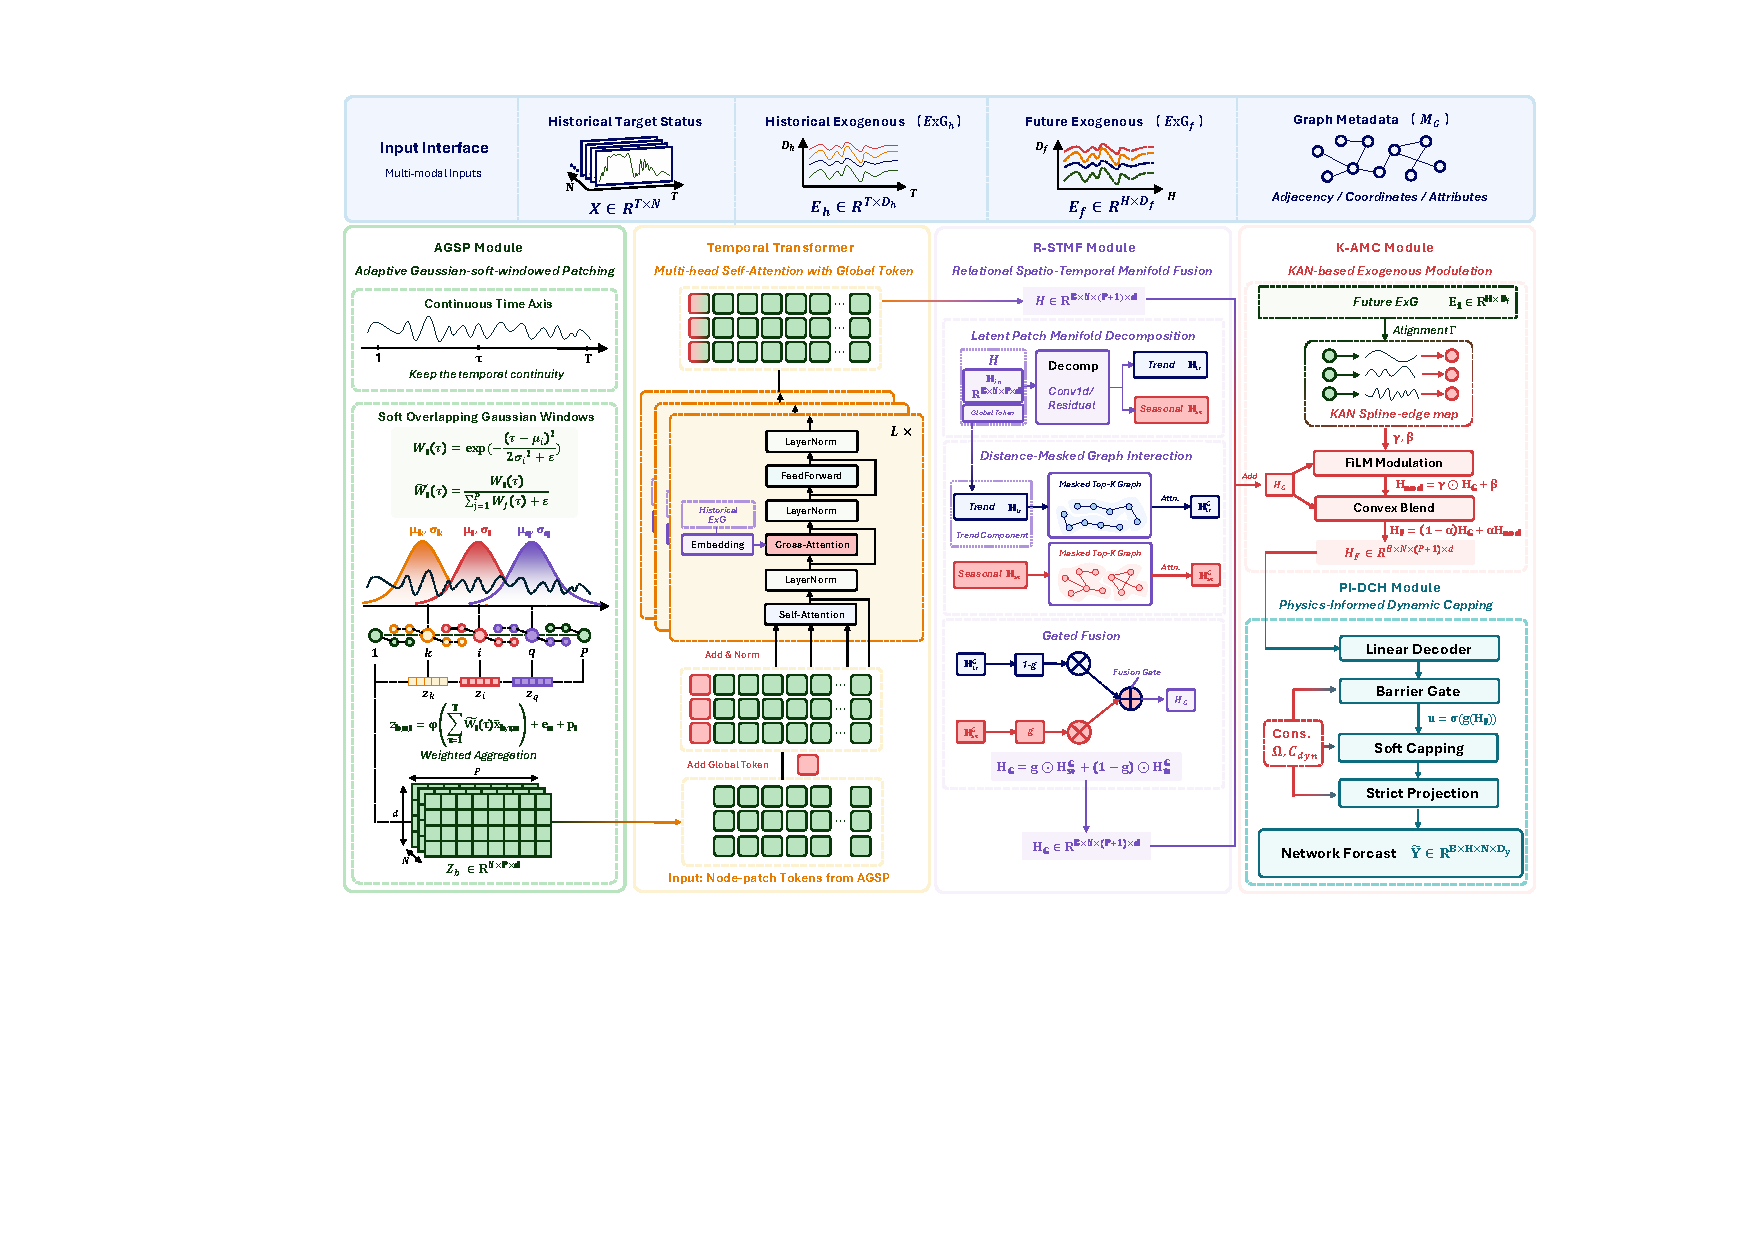
\includegraphics[width=\linewidth]{figures/Graph.pdf}
\caption{Overall architecture of PhyST-Net. The framework operates as an exogenous-aware vertical pipeline: (I) Multi-modal input interface; (II) AGSP continuous tokenization; (III) Transformer sequence encoding; (IV) R-STMF relational manifold fusion; (V) K-AMC spline-based conditioning; and (VI) PI-DCH domain-constrained forecasting. All external data (ExG and Metadata) and technical details are organized in peripheral tracks to ensure a clear and interpretable data flow.}
\label{fig:physt_architecture}
\end{figure*}


\subsection{Overall Framework}
\label{sec:overall_framework}
For a mini-batch, let $\mathbf{X}\in\mathbb{R}^{B\times T\times N\times D_x}$ denote historical target states, $\mathbf{E}^h\in\mathbb{R}^{B\times T\times D_h}$ denote historical ExG, and $\mathbf{E}^f\in\mathbb{R}^{B\times H\times D_f}$ denote future ExG. The model produces $\hat{\mathbf{Y}}\in\mathbb{R}^{B\times H\times N\times D_y}$. The computation can be written as
\begin{equation}
Z = \Phi_{patch}(\mathbf{X},\mathbf{E}^{h},M_G),
\label{eq:overall_patch}
\end{equation}
\begin{equation}
H_T = \Phi_{temp}(Z),\quad H_G = \Phi_{graph}(H_T,A,M_G),
\label{eq:overall_temp_graph}
\end{equation}
\begin{equation}
H_F = \Phi_{exg}(H_G,\mathbf{E}^{f}),\quad \hat{\mathbf{Y}} = \Phi_{head}(H_F,\mathbf{E}^{f},\Omega),
\label{eq:overall_exg_head}
\end{equation}
where $\Phi_{patch}$ is AGSP, $\Phi_{temp}$ is the temporal Transformer encoder, $\Phi_{graph}$ is the graph adapter (R-STMF), $\Phi_{exg}$ is future-ExG conditioning (K-AMC), and $\Phi_{head}$ is the physics-informed prediction head (PI-DCH). This decomposition emphasizes that the architectural backbone is defined on generic graph-structured sequences, while domain-specific knowledge is encapsulated in the input interface and the constraint head.

\subsection{Adaptive Gaussian-soft-windowed Patching}
\label{sec:agsp}
Transformer-based forecasters conventionally mitigate sequence length by aggregating observations into discrete temporal patches. While computationally convenient, fixed non-overlapping patches inevitably induce boundary artifacts when the underlying physical signal transverses a patch boundary. Aligning with emerging principles in complexity-balanced sequence modeling---where representational capacity is dynamically distributed proportional to signal variation---AGSP supersedes rigid patch assignments with learnable Gaussian soft-windows. This differentiable formulation empowers the architecture to autonomously allocate dense receptive fields to highly transient events and broader, smoother fields to stable operational regimes.

\begin{figure}[!t]
\centering
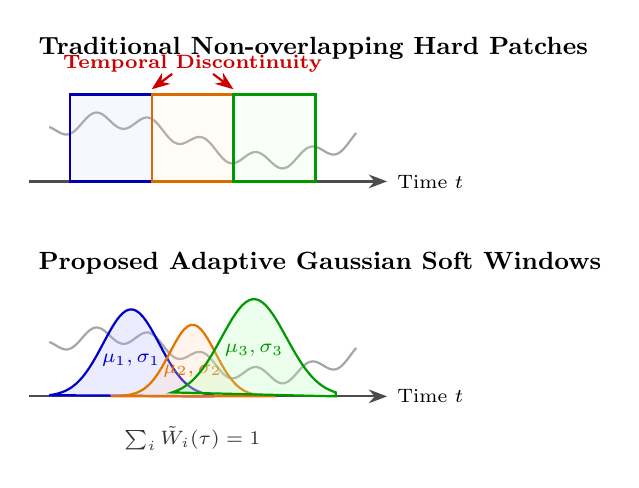
\begin{tikzpicture}[
    font=\rmfamily\scriptsize,
    >=Stealth,
    x=1.3cm, y=1.3cm,
    axis/.style={->, thick, draw=black!70},
    signal/.style={gray!70, thick},
    hard/.style={thick, fill opacity=0.15},
    soft/.style={thick, fill opacity=0.25},
    warn/.style={->, thick, draw=red!80!black},
    note/.style={font=\tiny, align=center}
]
    % (a) Rigid
    \begin{scope}[shift={(0, 2.1)}]
        \node[anchor=south west, font=\bfseries\small] at (0, 1.1) {Traditional Non-overlapping Hard Patches};
        \draw[axis] (0,0) -- (3.5,0) node[right] {Time $t$};
        \draw[signal] plot[domain=0.2:3.2, samples=100] (\x,{0.4 + 0.2*sin(deg(2*\x)) + 0.08*sin(deg(12*\x))});
        
        \draw[blue!70!black, hard, fill=blue!20] (0.4, 0) rectangle (1.2, 0.85);
        \draw[orange!85!black, hard, fill=orange!20] (1.2, 0) rectangle (2.0, 0.85);
        \draw[green!60!black, hard, fill=green!20] (2.0, 0) rectangle (2.8, 0.85);
        
        \node[text=red!80!black, font=\bfseries\scriptsize, align=center] (art1) at (1.6, 1.15) {Temporal Discontinuity};
        \draw[warn] (1.4, 1.05) -- (1.2, 0.9);
        \draw[warn] (1.8, 1.05) -- (2.0, 0.9);
    \end{scope}
    
    % (b) Soft
    \begin{scope}[shift={(0, 0)}]
        \node[anchor=south west, font=\bfseries\small] at (0, 1.1) {Proposed Adaptive Gaussian Soft Windows};
        \draw[axis] (0,0) -- (3.5,0) node[right] {Time $t$};
        \draw[signal] plot[domain=0.2:3.2, samples=100] (\x,{0.4 + 0.2*sin(deg(2*\x)) + 0.08*sin(deg(12*\x))});
        
        \path[fill=blue!30, draw=blue!80!black, soft] (0.2,0) plot[domain=0.2:1.8, samples=50] (\x,{0.85*exp(-((\x-1)^2)/0.15)}) -- (1.8,0) -- cycle;
        \node[blue!80!black, font=\scriptsize] at (1.0, 0.35) {$\mu_1, \sigma_1$};
        
        \path[fill=orange!30, draw=orange!90!black, soft] (0.8,0) plot[domain=0.8:2.4, samples=50] (\x,{0.7*exp(-((\x-1.6)^2)/0.1)}) -- (2.4,0) -- cycle;
        \node[orange!90!black, font=\scriptsize] at (1.6, 0.25) {$\mu_2, \sigma_2$};
        
        \path[fill=green!30, draw=green!60!black, soft] (1.4,0) plot[domain=1.4:3.0, samples=50] (\x,{0.95*exp(-((\x-2.2)^2)/0.2)}) -- (3.0,0) -- cycle;
        \node[green!60!black, font=\scriptsize] at (2.2, 0.45) {$\mu_3, \sigma_3$};
        
        \node[anchor=north, font=\scriptsize, text=black!80] at (1.6, -0.2) {$\sum_i \tilde{W}_i(\tau) = 1$};
    \end{scope}
\end{tikzpicture}
\caption{Mechanics of AGSP. By replacing discrete sequence chunking with continuous, differentiable density windows, the model autonomously mitigates boundary artifacts and preserves temporal continuity. Each soft window is parameterized by a learnable center $\mu_i$ and bandwidth $\sigma_i$, with overlapping weights dynamically normalized.}
\label{fig:agsp_detail}
\end{figure}

For node $n$ and temporal window $i$, the unnormalized weight at time index $\tau\in\{1,\ldots,T\}$ is
\begin{equation}
W_i(\tau)=\exp\left(-\frac{(\tau-\mu_i)^2}{2\sigma_i^2+\epsilon}\right),
\label{eq:agsp_window}
\end{equation}
where $\mu_i$ and $\sigma_i$ are learnable center and bandwidth parameters. To ensure numerical stability and valid window properties, we parameterize the bandwidth as $\sigma_i = \text{softplus}(\rho_i) + \delta$, where $\rho_i$ is the learnable parameter. The centers $\mu_i$ are initialized to uniform grid locations across the historical window to encourage an ordered temporal partition. The weights are normalized across $P$ windows:
\begin{equation}
\tilde{W}_i(\tau)=\frac{W_i(\tau)}{\sum_{j=1}^{P}W_j(\tau)+\epsilon}.
\label{eq:agsp_norm}
\end{equation}
Let $\bar{x}_{n}(\tau)$ denote the embedded historical state. The token for node $n$ and patch $i$ is
\begin{equation}
z_{n,i}=\psi\left(\sum_{\tau=1}^{T}\tilde{W}_i(\tau)\bar{x}_{n}(\tau)\right)+e_n+p_i,
\label{eq:agsp_token}
\end{equation}
where $\psi(\cdot)$ is a linear projection, $e_n$ is a node embedding, and $p_i$ is a temporal patch embedding.

\subsection{Temporal Representation Learning}
\label{sec:temporal_encoder}
Adopting the global token philosophy \cite{wang2024timexer} to facilitate efficient long-range context fusion, the token tensor $Z$ is concatenated with a learnable global token $z_{global} \in \mathbb{R}^{B \times N \times 1 \times d}$ for each node. This global token serves as a sequence-level memory bottleneck, aggregating the macroscopic temporal representation (e.g., shared external regimes or system-wide traffic trends) across all local patches. 

We denote the temporal encoding backbone as $\operatorname{STEnc}(\cdot)$. In PhyST-Net, rather than a naive standard Transformer, STEnc incorporates a targeted cross-attention mechanism. Specifically, within each encoder layer, the augmented node-wise token sequence $[Z \parallel z_{global}]$ first undergoes standard multi-head self-attention. Subsequently, to enrich the macro-trend representation with system-wide context, the global token uniquely cross-attends to the embedded historical exogenous features (e.g., SCADA and time-mark metadata), acting as an information sink:
\begin{equation}
z_{global}' = z_{global} + \operatorname{CrossAttention}(z_{global}, \mathbf{E}^h, \mathbf{E}^h).
\label{eq:cross_attention}
\end{equation}
This contextually enriched sequence is then processed through the feed-forward networks, yielding the final temporal representation:
\begin{equation}
H_T=\operatorname{STEnc}([Z \parallel z_{global}]), \quad H_T\in\mathbb{R}^{B\times N\times (P+1)\times d}.
\label{eq:temporal_encoder}
\end{equation}
Crucially, rather than discarding the global token post-encoding, PhyST-Net structurally leverages it to separate the node's state into two distinct manifolds: a local-variation patch state $U \triangleq H_{T,1:P}$ and a macro-trend global state $R \triangleq H_{T,P+1}$.

\subsection{Relational Spatio-Temporal Manifold Fusion (R-STMF)}
\label{sec:rstmf}
R-STMF serves as the graph adapter, specifically designed to capture the multi-modal spatial dependencies inherent in physical networks. Unlike conventional graph operators that treat node features as monolithic vectors, R-STMF recognizes that spatial interactions occur across different temporal scales within the latent space. To address this, we perform a \textbf{Latent Patch Manifold Decomposition}.

Let $H_{in} = H_T$ denote the input latent representation. For each node $n$, we apply a 1D depth-wise convolution along the patch dimension to extract the smoothed trend component $H_{tr}$, while the residual represents the seasonal (oscillatory) component $H_{se}$:
\begin{align}
H_{tr} &= \operatorname{GELU}(\operatorname{Conv1d}(H_{in})), \label{eq:rstmf_decomp_tr} \\
H_{se} &= H_{in} - H_{tr}. \label{eq:rstmf_decomp_se}
\end{align}

\begin{figure*}[!t]
\centering
\resizebox{\textwidth}{!}{%
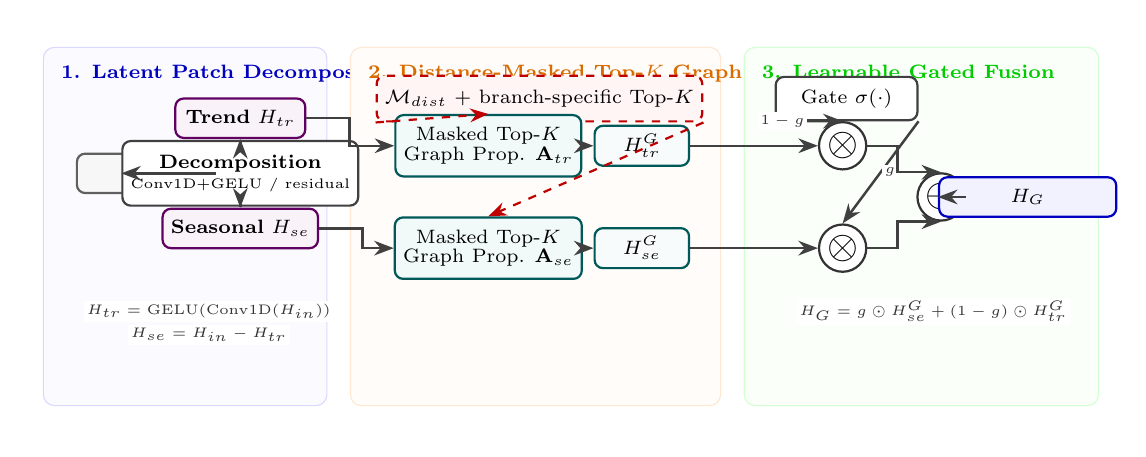
\begin{tikzpicture}[
    font=\rmfamily\scriptsize,
    >=Stealth,
    x=1.0cm, y=1.0cm,
    module/.style={
        draw=black!75,
        rounded corners=3pt,
        thick,
        align=center,
        fill=white,
        inner sep=3pt
    },
    state/.style={
        module,
        fill=blue!5,
        draw=blue!75!black,
        minimum width=1.55cm,
        minimum height=0.50cm
    },
    branch/.style={
        module,
        fill=violet!5,
        draw=violet!75!black,
        minimum width=1.65cm,
        minimum height=0.50cm
    },
    graph/.style={
        module,
        fill=teal!5,
        draw=teal!70!black,
        minimum width=2.00cm,
        minimum height=0.78cm
    },
    mask/.style={
        module,
        fill=red!4,
        draw=red!75!black,
        dashed,
        minimum width=2.35cm,
        minimum height=0.58cm
    },
    op/.style={
        circle,
        draw=black!80,
        thick,
        fill=white,
        minimum size=6.0mm,
        inner sep=0pt
    },
    arrow/.style={
        ->,
        line width=0.90pt,
        draw=black!75
    },
    maskarrow/.style={
        ->,
        dashed,
        line width=0.80pt,
        draw=red!75!black
    },
    lab/.style={
        font=\tiny,
        fill=white,
        inner sep=1.1pt,
        text=black!80
    },
    title/.style={
        anchor=north west,
        font=\bfseries\scriptsize
    }
]

% ---------------------------------------------------------
% Canvas and background panels
% ---------------------------------------------------------
\path[use as bounding box] (-0.55,-0.85) rectangle (13.30,4.25);

\draw[fill=blue!2, draw=blue!15, rounded corners=4pt]
    (-0.35,-0.55) rectangle (3.25,4.00);
\node[title, text=blue!75!black] at (-0.25,3.90)
    {1. Latent Patch Decomposition};

\draw[fill=orange!2, draw=orange!18, rounded corners=4pt]
    (3.55,-0.55) rectangle (8.25,4.00);
\node[title, text=orange!85!black] at (3.65,3.90)
    {2. Distance-Masked Top-$K$ Graph Interaction};

\draw[fill=green!2, draw=green!18, rounded corners=4pt]
    (8.55,-0.55) rectangle (13.05,4.00);
\node[title, text=green!80!black] at (8.65,3.90)
    {3. Learnable Gated Fusion};

% ---------------------------------------------------------
% Stage 1: decomposition
% ---------------------------------------------------------
\node[state, fill=gray!6, draw=gray!75!black, minimum width=1.75cm]
    (hin) at (0.95,2.40) {\textbf{$H_{in}$}};

\node[module, minimum width=1.95cm, minimum height=0.82cm]
    (decomp) at (2.15,2.40)
    {\textbf{Decomposition}\\[-1pt]
    {\tiny Conv1D+GELU / residual}};

\node[branch] (htr) at (2.15,3.10)
    {\textbf{Trend} $H_{tr}$};

\node[branch] (hse) at (2.15,1.70)
    {\textbf{Seasonal} $H_{se}$};

\draw[arrow] (hin.east) -- (decomp.west);
\draw[arrow] (decomp.north) -- (htr.south);
\draw[arrow] (decomp.south) -- (hse.north);

\node[lab] at (1.75,0.65)
    {$H_{tr}=\mathrm{GELU}(\mathrm{Conv1D}(H_{in}))$};
\node[lab] at (1.75,0.35)
    {$H_{se}=H_{in}-H_{tr}$};

% ---------------------------------------------------------
% Stage 2: graph interaction
% ---------------------------------------------------------
\node[mask] (mask) at (5.95,3.35)
    {$\mathcal{M}_{dist}$ + branch-specific Top-$K$};

\node[graph] (gtr) at (5.30,2.75)
    {Masked Top-$K$\\[-1pt]
    Graph Prop. $\mathbf{A}_{tr}$};

\node[graph] (gse) at (5.30,1.45)
    {Masked Top-$K$\\[-1pt]
    Graph Prop. $\mathbf{A}_{se}$};

\node[state, fill=teal!3, draw=teal!70!black, minimum width=1.20cm]
    (hgtr) at (7.25,2.75) {$H_{tr}^{G}$};

\node[state, fill=teal!3, draw=teal!70!black, minimum width=1.20cm]
    (hgse) at (7.25,1.45) {$H_{se}^{G}$};

\draw[arrow] (htr.east) -- ++(0.55,0) |- (gtr.west);
\draw[arrow] (hse.east) -- ++(0.55,0) |- (gse.west);

\draw[arrow] (gtr.east) -- (hgtr.west);
\draw[arrow] (gse.east) -- (hgse.west);

% short mask injection arrows
\draw[maskarrow] (mask.south west) -- (gtr.north);
\draw[maskarrow] (mask.south east) -- (gse.north);

% ---------------------------------------------------------
% Stage 3: gated fusion
% ---------------------------------------------------------
\node[module, minimum width=1.80cm, minimum height=0.55cm]
    (gate) at (9.85,3.35)
    {Gate $\sigma(\cdot)$};

\node[op] (multr) at (9.80,2.75) {\Large $\otimes$};
\node[op] (mulse) at (9.80,1.45) {\Large $\otimes$};

\node[op] (add) at (11.05,2.10) {\Large $\oplus$};

\node[state, minimum width=2.25cm]
    (hg) at (12.15,2.10)
    {\textbf{$H_G$}};

\draw[arrow] (hgtr.east) -- (multr.west);
\draw[arrow] (hgse.east) -- (mulse.west);

\draw[arrow] (gate.south west) -- (multr.north)
    node[midway, left, lab] {$1-g$};

\draw[arrow] (gate.south east) -- (mulse.north)
    node[midway, right, lab] {$g$};

\draw[arrow] (multr.east) -- ++(0.38,0) |- (add.north);
\draw[arrow] (mulse.east) -- ++(0.38,0) |- (add.south);
\draw[arrow] (add.east) -- (hg.west);

\node[lab] at (10.95,0.65)
    {$H_G=g\odot H_{se}^{G}+(1-g)\odot H_{tr}^{G}$};

\end{tikzpicture}
}
\caption{Detailed architecture of R-STMF. The latent representation is decomposed into trend and seasonal manifolds. Each branch performs distance-masked Top-$K$ graph propagation with branch-specific routing, and the resulting graph-enhanced manifolds are fused through a learnable gate.}
\label{fig:rstmf_detail}
\end{figure*}

This decomposition ensures that the model can independently learn how macro-scale trends and micro-scale seasonal fluctuations propagate through the graph.

\subsubsection{Distance-Masked Relational Pruning}
For each manifold $c \in \{se, tr\}$, we compute relational attention scores across nodes. To enforce physical realism and reduce computational overhead, we introduce a \textbf{Distance-Masked Top-$K$ Pruning} strategy. Given a physical distance matrix or prior topology, we define a binary mask $\mathcal{M}_{dist}$, where $\mathcal{M}_{ij}=1$ only if node $j$ is within a feasible interaction radius of node $i$. The masked attention score $S_c$ is:
\begin{equation}
\resizebox{0.88\hsize}{!}{$
S_{c,ij} = \begin{cases} \frac{Q_c(K_c)^{\top}}{\sqrt{d_m}} & \text{if } \mathcal{M}_{ij}=1 \\ -\infty & \text{otherwise} \end{cases}, \quad A_c=\operatorname{Softmax}\left(\operatorname{TopK}(S_c, K_c)\right).
$}
\label{eq:rstmf_routing}
\end{equation}
Subsequently, we perform Top-$K$ selection on the remaining scores to ensure a sparse and robust graph routing. Finally, the graph-enhanced seasonal and trend manifolds are recombined using a learnable gated fusion mechanism:
\begin{align}
g &= \sigma(\operatorname{Linear}([H_{se}^G \parallel H_{tr}^G])), \\
H_G &= g \odot H_{se}^G + (1-g) \odot H_{tr}^G,
\label{eq:rstmf_fusion}
\end{align}
where $H_{c}^G$ denotes the manifold $c$ after spatial propagation via $A_c$. This dual-branch architecture allows PhyST-Net to model complex spatio-temporal interactions without conflating multi-resolution physical mechanisms.

\subsection{Future-ExG Conditioning (K-AMC)}
\label{sec:kamc}
We refer to this module as K-AMC, short for KAN-enhanced Adaptive Modulation and Conditioning. It serves as a generalized interface for known systemic drivers, injecting future exogenous drivers $\mathbf{E}^f \in \mathbb{R}^{B \times H \times D_f}$ into the latent representations. Aligning with the TimeXer philosophy \cite{wang2024timexer}, the macro-trend global token acts as the primary bridge to cross-attend and ingest external factors. We define an alignment operator $\Gamma$ that maps the future horizon into variate tokens corresponding to the latent states.

\begin{figure*}[!t]
\centering
\resizebox{\textwidth}{!}{%
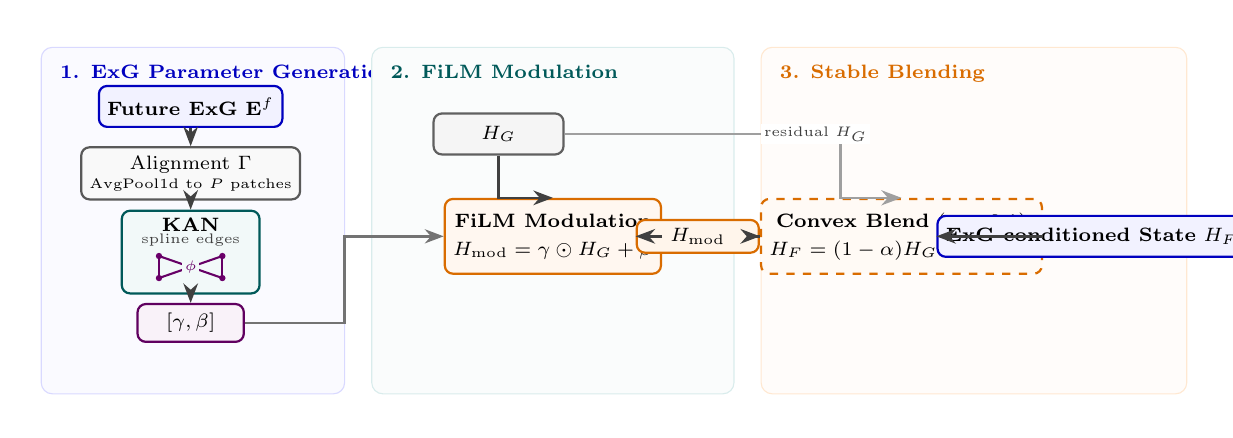
\begin{tikzpicture}[
    font=\rmfamily\scriptsize,
    >=Stealth,
    x=1.15cm, y=1.00cm,
    module/.style={
        draw=black!75,
        rounded corners=3pt,
        thick,
        align=center,
        fill=white,
        inner sep=3pt
    },
    input/.style={
        module,
        fill=blue!5,
        draw=blue!75!black,
        minimum width=2.10cm,
        minimum height=0.52cm
    },
    process/.style={
        module,
        fill=gray!5,
        draw=black!65,
        minimum width=2.15cm,
        minimum height=0.58cm
    },
    kan/.style={
        module,
        fill=teal!5,
        draw=teal!70!black,
        minimum width=1.75cm,
        minimum height=1.05cm
    },
    param/.style={
        module,
        fill=violet!5,
        draw=violet!75!black,
        minimum width=1.35cm,
        minimum height=0.48cm
    },
    film/.style={
        module,
        fill=orange!6,
        draw=orange!85!black,
        minimum width=2.65cm,
        minimum height=0.95cm
    },
    blend/.style={
        module,
        fill=orange!4,
        draw=orange!85!black,
        dashed,
        minimum width=3.15cm,
        minimum height=0.95cm
    },
    arrow/.style={
        ->,
        line width=0.9pt,
        draw=black!75
    },
    auxarrow/.style={
        ->,
        line width=0.85pt,
        draw=black!55
    },
    residual/.style={
        ->,
        line width=0.95pt,
        draw=gray!75
    },
    title/.style={
        anchor=north west,
        font=\bfseries\scriptsize
    },
    note/.style={
        font=\tiny,
        align=center,
        text=black!75
    }
]

% ---------------------------------------------------------
% Canvas and background panels
% ---------------------------------------------------------
\path[use as bounding box] (-0.45,-0.65) rectangle (12.55,4.20);

\draw[fill=blue!2, draw=blue!15, rounded corners=4pt]
    (-0.30,-0.45) rectangle (3.05,3.95);
\node[title, text=blue!75!black] at (-0.20,3.85)
    {1. ExG Parameter Generation};

\draw[fill=teal!2, draw=teal!15, rounded corners=4pt]
    (3.35,-0.45) rectangle (7.35,3.95);
\node[title, text=teal!70!black] at (3.45,3.85)
    {2. FiLM Modulation};

\draw[fill=orange!2, draw=orange!18, rounded corners=4pt]
    (7.65,-0.45) rectangle (12.35,3.95);
\node[title, text=orange!85!black] at (7.75,3.85)
    {3. Stable Blending};

% ---------------------------------------------------------
% Stage 1: ExG parameter generation
% ---------------------------------------------------------
\node[input] (ef) at (1.35,3.20)
    {\textbf{Future ExG} $\mathbf{E}^{f}$};

\node[process] (align) at (1.35,2.35)
    {Alignment $\Gamma$\\[-1pt]
    {\tiny AvgPool1d to $P$ patches}};

\node[kan] (kanblk) at (1.35,1.35) {};

\node[font=\bfseries\scriptsize] at (1.35,1.70) {KAN};
\node[note] at (1.35,1.50) {spline edges};

% compact KAN internal edge diagram
\coordinate (u1) at (1.00,1.30);
\coordinate (u2) at (1.70,1.30);
\coordinate (v1) at (1.00,1.02);
\coordinate (v2) at (1.70,1.02);

\fill[violet!85!black] (u1) circle (1.15pt);
\fill[violet!85!black] (u2) circle (1.15pt);
\fill[violet!85!black] (v1) circle (1.15pt);
\fill[violet!85!black] (v2) circle (1.15pt);

\draw[violet!80!black, line width=0.75pt] (u1) -- (v1);
\draw[violet!80!black, line width=0.75pt] (u2) -- (v2);
\draw[violet!80!black, line width=0.75pt] (u1) -- (v2);
\draw[violet!80!black, line width=0.75pt] (u2) -- (v1);

\node[violet!80!black, font=\tiny, fill=teal!5, inner sep=1pt]
    at (1.35,1.16) {$\phi$};

\node[param] (params) at (1.35,0.45)
    {$[\gamma,\beta]$};

\draw[arrow] (ef.south) -- (align.north);
\draw[arrow] (align.south) -- (kanblk.north);
\draw[arrow] (kanblk.south) -- (params.north);

% ---------------------------------------------------------
% Stage 2: FiLM modulation
% ---------------------------------------------------------
\node[input, fill=gray!8, draw=gray!75!black, minimum width=1.65cm]
    (hg) at (4.75,2.85) {\textbf{$H_G$}};

\node[film] (film) at (5.35,1.55)
    {\textbf{FiLM Modulation}\\[2pt]
    $H_{\mathrm{mod}}=\gamma\odot H_G+\beta$};

\node[module, fill=orange!8, draw=orange!85!black, minimum width=1.55cm]
    (hmod) at (6.95,1.55) {\textbf{$H_{\mathrm{mod}}$}};

\draw[arrow] (hg.south) |- (film.north);
\draw[auxarrow] (params.east) -- ++(1.10,0) |- (film.west);
\draw[arrow] (film.east) -- (hmod.west);

% ---------------------------------------------------------
% Stage 3: Convex blending
% ---------------------------------------------------------
\node[blend] (blend) at (9.20,1.55)
    {\textbf{Convex Blend} $(\alpha=0.1)$\\[2pt]
    $H_F=(1-\alpha)H_G+\alpha H_{\mathrm{mod}}$};

\node[input, minimum width=2.95cm]
    (hf) at (11.30,1.55)
    {\textbf{ExG-conditioned State} $H_F$};

\draw[arrow] (hmod.east) -- (blend.west);
\draw[arrow] (blend.east) -- (hf.west);

% residual path from H_G to blend, routed above
\draw[residual] (hg.east) -- ++(3.05,0) |- (blend.north);
\node[note, fill=white, inner sep=1pt] at (8.25,2.85)
    {residual $H_G$};

\end{tikzpicture}
}
\caption{Mechanics of K-AMC. Future exogenous drivers are aligned to the patch scale and processed by a compact KAN block to generate dynamic modulation parameters. The graph-enhanced state is first modulated by FiLM and then stabilized through convex blending with the original state.}
\label{fig:kamc_detail}
\end{figure*}

The aligned representation $\bar{\mathbf{E}}^f$ is then passed through a Kolmogorov-Arnold Network (KAN) block. Unlike standard MLPs, KANs parameterize transformations using learnable univariate B-spline functions on the edges. For an input feature $x$, the edge function is defined as:
\begin{equation}
\phi(x) = w_b \operatorname{SiLU}(x) + \sum_{i=1}^{k} c_i B_i(x),
\label{eq:kan_edge_sum}
\end{equation}
where $B_i(x)$ are B-spline basis functions. The analytical derivative is:
\begin{equation}
\frac{\partial \phi(x)}{\partial x} = w_b \operatorname{SiLU}'(x) + \sum_{i=1}^{k} c_i B'_i(x).
\label{eq:kan_derivative}
\end{equation}
By aggregating these edge functions, the KAN block produces modulation parameters $[\gamma,\beta]=\operatorname{KAN}(\bar{\mathbf{E}}^f)$. The final conditioned latent state is then obtained via element-wise scale and shift, stabilized by a convex blending scheme with hyperparameter $\alpha=0.1$:
\begin{equation}
H_{mod} = \gamma \odot H_G + \beta, \quad H_F = (1-\alpha)H_G + \alpha H_{mod}.
\label{eq:kamc_mod}
\end{equation}

\subsection{Physics-Informed Dynamic Capping Head (PI-DCH)}
\label{sec:pidch}
PI-DCH instantiates the constraint operator $\mathcal{C}_{\Omega}$. In mission-critical environments such as smart grids, safety-critical traffic routing, and industrial control systems, deploying predictive models mandates rigorous output-space guidance to preclude physically unfeasible trajectories. While hard projection operators (e.g., clipping) guarantee bounded outputs, they may create a mismatch between training and inference, and can severely weaken gradient signals when used naively, hampering the learning process.

To ensure that the model remains physically consistent even under extreme scenarios, we adopt a dual-stage enforcement strategy. While $\hat{Y}_{soft}=\tilde{Y}+u\odot(C_{dyn}-\tilde{Y})$ provides the differentiable path necessary for optimization via a learned barrier gate $u=\sigma(g(H_F))$, we define the final deployment-ready forecast $\hat{\mathbf{Y}}$ through a \textbf{Strict Operational Boundary Enforcement} layer:
\begin{equation}
\hat{\mathbf{Y}} = \operatorname{Proj}_{\mathcal{K}}(\hat{Y}_{soft}) \triangleq \max(0, \min(\hat{Y}_{soft}, C_{dyn})),
\label{eq:pidch_enforcement}
\end{equation}
where $\operatorname{Proj}_{\mathcal{K}}$ denotes the Euclidean projection onto the dynamic feasible set $\mathcal{K} = [0, C_{dyn}]$. Crucially, this projection is treated as a non-trainable safety layer during inference to guarantee 100\% compliance with physical limits. By decoupling the differentiable steering ($\hat{Y}_{soft}$) from the strict enforcement ($\hat{\mathbf{Y}}$), PhyST-Net achieves the dual goals of stable gradient backpropagation and absolute operational feasibility.

\subsection{Computational Complexity Analysis}
\label{sec:complexity_analysis}
A core motivation of PhyST-Net is mitigating the severe computational bottlenecks of dense spatio-temporal Transformers, which conventionally exhibit a time complexity of $\mathcal{O}(N \cdot T^2 + T \cdot N^2)$ for sequence length $T$ and node count $N$. PhyST-Net structurally resolves this through its decoupled topology.

In the temporal pathway, the AGSP module compresses the raw $T$-length sequence into $P$ continuous tokens (where $P \ll T$). Consequently, the temporal Transformer encoder's self-attention complexity is reduced from $\mathcal{O}(N \cdot T^2)$ to $\mathcal{O}(N \cdot P^2)$. 

In the spatial pathway, standard full-graph attention requires $\mathcal{O}(P \cdot N^2)$ operations. The R-STMF module introduces a Top-$K$ sparse masking strategy (Eq.~\ref{eq:rstmf_routing}), restricting message passing to a parameterized neighborhood size $K$. This bounds the spatial complexity to $\mathcal{O}(P \cdot K \cdot N)$. Thus, the overall self-attention complexity of the PhyST-Net backbone is decoupled and bounded by $\mathcal{O}(N \cdot P^2 + P \cdot K \cdot N)$, rendering the architecture highly scalable for large physical networks and extended forecasting horizons without sacrificing expressive capability.

\subsection{Optimization Objective}
\label{sec:optimization}
To bridge the gap between purely data-driven forecasting and physical feasibility, we minimize a multi-objective loss $\mathcal{L} = \mathcal{L}_{mae} + \lambda_{\Omega}\mathcal{L}_{penalty}$. The penalty term $\mathcal{L}_{penalty}$ structurally regularizes the model to internalize the operational set $\Omega$ during backpropagation. Utilizing the positive-part operator $[x]^+ \triangleq \max(0, x)$, we decouple the penalty into two physically meaningful components: a non-negativity constraint and a dynamic capacity limit constraint:
\begin{align}
\mathcal{L}_{penalty} &= \mathcal{L}_{neg} + \mathcal{L}_{cap}, \label{eq:feasibility_penalty_total} \\
\mathcal{L}_{neg} &= \frac{1}{|\mathcal{D}|HN} \sum_{\mathcal{D}} \sum_{n,h} [-\hat{Y}_{soft,n,h}]^+, \label{eq:feasibility_penalty_neg} \\
\mathcal{L}_{cap} &= \frac{1}{|\mathcal{D}|HN} \sum_{\mathcal{D}} \sum_{n,h} [\hat{Y}_{soft,n,h} - C_{dyn,n,h}]^+. \label{eq:feasibility_penalty_cap}
\end{align}
This decoupled formulation ensures the model learns to respect physical boundaries natively, thereby reducing the reliance on reactive clipping at inference time. The overall training logic is summarized in Algorithm~\ref{alg:physt_net}.

\begin{algorithm}[!t]
\caption{PhyST-Net Forward Pass}
\label{alg:physt_net}
\begin{algorithmic}[1]
\REQUIRE Input tuple $\mathcal{X}_t = (\mathbf{X}, \mathbf{E}^h, \mathbf{E}^f, A, M_G)$, Domain knowledge $\Omega$.
\ENSURE Feasible network forecast $\hat{\mathbf{Y}}$.

\STATE \COMMENT{\textit{Phase I: AGSP Continuous Tokenization}}
\STATE Initialize learnable Gaussian parameters $\mu_i, \sigma_i$ for $P$ tokens using metadata $M_G$.
\FOR{each token $i \in \{1,\ldots,P\}$}
    \STATE Compute soft-window weights $W_i(\tau) = \exp\left(-\frac{(\tau-\mu_i)^2}{2\sigma_i^2+\epsilon}\right)$.
    \STATE Aggregate $\mathbf{X}$ and $\mathbf{E}^h$ via $W_i(\tau)$ to form continuous token $Z_{:,i,:}$.
\ENDFOR

\STATE \COMMENT{\textit{Phase II: Temporal Encoding ($\mathcal{H}_\theta$ part 1)}}
\STATE Process $Z$ via Multi-Head Self-Attention to capture temporal dependencies $\to H_T$.

\STATE \COMMENT{\textit{Phase III: R-STMF Graph Adaptation ($\mathcal{H}_\theta$ part 2)}}
\STATE Decompose $H_{in} = H_T$ into seasonal $H_{se}$ and trend $H_{tr}$ manifolds.
\STATE Apply Top-$K$ sparse masking to $A$ based on spatial similarities and physical distances.
\STATE Propagate $H_{se}$ and $H_{tr}$ over the masked graph and fuse $\to H_G$.

\STATE \COMMENT{\textit{Phase IV: K-AMC Exogenous Modulation ($\mathcal{H}_\theta$ part 3)}}
\STATE Align horizon-wise $\mathbf{E}^f$ to patch-wise representation $\bar{\mathbf{E}}^f$.
\STATE Compute B-spline edge functions via KAN block to generate $[\gamma, \beta]$.
\STATE Modulate latent states: $H_F \leftarrow (1-\alpha)H_G + \alpha(\gamma \odot H_G + \beta)$.

\STATE \COMMENT{\textit{Phase V: PI-DCH Constraint Decoding ($\mathcal{C}_\Omega$)}}
\STATE Decode unconstrained prediction $\tilde{Y} = \operatorname{Linear}(H_F)$.
\STATE Shape prediction softly: $\hat{Y}_{soft} \leftarrow \tilde{Y} + u \odot (C_{dyn} - \tilde{Y})$.
\STATE Project to feasible set: $\hat{\mathbf{Y}} \leftarrow \operatorname{Proj}_{\mathcal{K}}(\hat{Y}_{soft})$.

\RETURN $\hat{\mathbf{Y}}$.
\end{algorithmic}
\end{algorithm}

\section{Experiments}
\label{sec:experiments}
% TODO: Experimental setup, dataset details, baseline comparisons, and ablation studies will be added here.
\section{Discussion and Qualitative Analysis}
\label{sec:discussion}
The reported results support the view that PhyST-Net is best understood as an ExG-aware spatio-temporal graph Transformer with a wind-specific physical instantiation. This section discusses the modeling implications, optimization effects, and the remaining validation gaps.

\subsection{Optimization Effect of Relational Pruning}
\label{sec:pruning_discussion}
The relational pruning strategy in R-STMF is not merely a computational heuristic for large graphs; it is a fundamental denoising mechanism. In wind farms, especially those in complex terrain (e.g., the HoT site), SCADA data often contains spurious cross-turbine correlations caused by sensor noise or localized turbulence that does not represent the macro wind field. By enforcing Top-$K$ sparsity, R-STMF forces the model to ignore these low-magnitude, high-frequency dependencies. 

Our preliminary analysis (see Fig.~\ref{fig:pruning_effect_placeholder}) suggests that as $K$ decreases, the model's stability during long-horizon forecasts improves. When $K$ is too large (approaching dense attention), the model tends to "over-smooth" the node-level states, losing the specific high-resolution details of individual turbine responses. Conversely, an optimally pruned graph adapter captures the essential propagation pathways—the "spatial backbone" of the wind farm—while maintaining a low computational footprint. This behavior aligns with the physical intuition that wind information propagates along dominant streamlines rather than diffusing uniformly across the entire farm.

\subsection{ExG as a Model Interface}
\label{sec:exg_interface_discussion}
A key design choice is to make exogenous variables explicit. Historical SCADA variables and future NWP-like variables serve different roles: the former explains recent operating context, while the latter conditions the forecast horizon. By separating historical ExG from future ExG, PhyST-Net avoids treating all covariates as a single feature block. This design is important for WPF, but it is also relevant to other graph forecasting tasks where future external drivers are known or forecast, such as traffic calendars, load schedules, weather forecasts, or planned control signals.

\subsection{Interpretability and Efficiency Trade-offs in K-AC}
\label{sec:kac_tradeoff}
K-AC introduces KAN-based modulation, which offers a unique trade-off between expressive power and transparency. While traditional MLPs can approximate any function, their ``black-box'' nature makes it difficult for operators to trust the model's reaction to extreme exogenous forecasts. KAN's additive spline structure allows for a feature-wise decomposition: one can visualize exactly how a 20\% increase in a forecast driver scales the latent node representations.

However, this interpretability comes at a cost. Evaluating B-splines is more computationally intensive than simple matrix multiplications, especially when the number of spline bases $M$ or the input dimension $D_f$ is large. In our complexity analysis (Section~\ref{sec:complexity}), we noted that K-AC's cost scales with $M$. In practice, we found that a small $M$ (e.g., 3 to 5) is often sufficient to capture the relevant operating regimes without significantly impacting inference latency. This suggests that K-AC is most effective when used as a ``surgical'' conditioning module rather than a replacement for all dense layers in the network.

\subsection{Aesthetic and Structural Integrity of the Forecast}
\label{sec:forecast_integrity}
Beyond numerical metrics like RMSE and MAE, the ``integrity'' of the forecast---its physical or operational plausibility---is crucial for decision-making. Standard STGNNs often produce ``jittery'' forecasts or predictions that exceed the physical capacity of the node during extreme events. DI-DCH addresses this by injecting the capacity envelope directly into the decoding process. This ensures that the generated time series is not only accurate on average but also structurally sound: it respects non-negativity and does not exceed rated limits. Such structural consistency reduces the need for heuristic post-processing and makes the model output directly compatible with downstream optimization tools.

\subsection{Temporal Continuity in Tokenization}
\label{sec:tokenization_role}
Adaptive Gaussian-soft-windowed Patching (AGSP) provides a continuous alternative to hard temporal segmentation. The validation on small-scale networks supports its value, while larger datasets show mixed results under current runs. This suggests that AGSP should be interpreted as a tokenization mechanism that can reduce boundary artifacts and improve smooth event representation. By allowing the temporal receptive fields to overlap and adapt, the model can ``track'' moving fronts across tokens more effectively than fixed-window methods.

\subsection{Generalization and Future Work}
\label{sec:future_work}
The proposed formulation is designed to be general-purpose. Candidate applications include traffic flow forecasting, electric load forecasting, photovoltaic generation, air-quality prediction, and distributed industrial sensing. 

Several avenues remain for future exploration. First, while K-AC provides a path toward interpretability, a more rigorous causal analysis of the learned spline functions would strengthen the grounding of the model. Second, the current version of PhyST-Net is a point-forecasting model; extending it to produce probabilistic intervals is essential for risk-aware operation. Finally, investigating the model's robustness to exogenous uncertainty---specifically how errors in future ExG propagate through the K-AC modulation---will be critical for real-world deployment.

\section{Case Studies}
\label{sec:case_studies}
% TODO: Visualizations of attention maps, dynamic constraint clipping, and specific forecasting cases will be added here.

\section{Conclusion}
\label{sec:conclusion}
\textbf{[Placeholder: Write the final conclusion after the experimental section is complete.]}

The final conclusion should summarize the problem setting, the ExG-aware STGT formulation, the roles of AGSP, R-STMF, K-AC, and DI-DCH, and the main validated findings from SDWPF, HoT, and Kelmarsh. It should also state the remaining limitations, such as cross-domain transfer, operational uncertainty, probabilistic forecasting, and larger-scale deployment.

% Generated by IEEEtran.bst, version: 1.14 (2015/08/26)
\begin{thebibliography}{10}
\providecommand{\url}[1]{#1}
\csname url@samestyle\endcsname
\providecommand{\newblock}{\relax}
\providecommand{\bibinfo}[2]{#2}
\providecommand{\BIBentrySTDinterwordspacing}{\spaceskip=0pt\relax}
\providecommand{\BIBentryALTinterwordstretchfactor}{4}
\providecommand{\BIBentryALTinterwordspacing}{\spaceskip=\fontdimen2\font plus
\BIBentryALTinterwordstretchfactor\fontdimen3\font minus
  \fontdimen4\font\relax}
\providecommand{\BIBforeignlanguage}[2]{{%
\expandafter\ifx\csname l@#1\endcsname\relax
\typeout{** WARNING: IEEEtran.bst: No hyphenation pattern has been}%
\typeout{** loaded for the language `#1'. Using the pattern for}%
\typeout{** the default language instead.}%
\else
\language=\csname l@#1\endcsname
\fi
#2}}
\providecommand{\BIBdecl}{\relax}
\BIBdecl

\bibitem{vaswani2017attention}
A.~Vaswani \emph{et al.}, ``Attention is all you need,'' in \emph{Advances in Neural Information Processing Systems}, 2017, pp. 5998--6008.

\bibitem{zhou2021informer}
H.~Zhou \emph{et al.}, ``{Informer}: Beyond efficient transformer for long sequence time-series forecasting,'' in \emph{Proceedings of the AAAI Conference on Artificial Intelligence}, vol.~35, no.~12, 2021, pp. 11\,106--11\,115.

\bibitem{wu2021autoformer}
H.~Wu \emph{et al.}, ``{Autoformer}: Decomposition transformers with auto-correlation for long-term series forecasting,'' in \emph{Advances in Neural Information Processing Systems}, vol.~34, 2021, pp. 22\,419--22\,430.

\bibitem{zhou2022fedformer}
T.~Zhou \emph{et al.}, ``{FEDformer}: Frequency enhanced decomposed transformer for long-term series forecasting,'' in \emph{International Conference on Machine Learning}, 2022, pp. 27\,268--27\,286.

\bibitem{nie2023patchtst}
Y.~Nie \emph{et al.}, ``A time series is worth 64 words: Long-term forecasting with transformers,'' in \emph{International Conference on Learning Representations (ICLR)}, 2023.

\bibitem{liu2024itransformer}
Y.~Liu \emph{et al.}, ``{iTransformer}: Inverted transformers are effective for time series forecasting,'' in \emph{International Conference on Learning Representations (ICLR)}, 2024.

\bibitem{kipf2017semi}
T.~N. Kipf and M.~Welling, ``Semi-supervised classification with graph convolutional networks,'' in \emph{International Conference on Learning Representations (ICLR)}, 2017.

\bibitem{velickovic2018graph}
P.~Veli{\v{c}}kovi{\'{c}} \emph{et al.}, ``Graph attention networks,'' in \emph{International Conference on Learning Representations (ICLR)}, 2018.

\bibitem{yu2017spatio}
B.~Yu, H.~Yin, and Z.~Zhu, ``Spatio-temporal graph convolutional networks: A deep learning framework for traffic forecasting,'' \emph{arXiv preprint arXiv:1709.04875}, 2017.

\bibitem{wu2019graph}
Z.~Wu \emph{et al.}, ``Graph wavenet for deep spatial-temporal graph modeling,'' \emph{arXiv preprint arXiv:1906.00121}, 2019.

\bibitem{li2024sdg}
X.~Li, Y.~Qiao, Z.~Li, and P.~Lu, ``{SDG-WindNet}: A spatio-temporal dual-graph network for wind speed prediction,'' \emph{IEEE Transactions on Power Systems}, 2024.

\bibitem{conformer2025}
M.~Li \emph{et al.}, ``Towards resilient transportation: A conditional transformer for accident-informed traffic forecasting,'' \emph{arXiv preprint arXiv:2512.09398}, 2025.

\bibitem{exost2025}
Y.~Zhang \emph{et al.}, ``Select, then balance: Exploring exogenous variable modeling of spatio-temporal forecasting,'' \emph{arXiv preprint arXiv:2509.05779}, 2025.

\bibitem{wang2024timexer}
Y.~Wang \emph{et al.}, ``TimeXer: Empowering transformers for time series forecasting with exogenous variables,'' in \emph{Advances in Neural Information Processing Systems}, 2024.

\bibitem{dag2025}
Z.~Chen \emph{et al.}, ``DAG: A dual correlation network for time series forecasting with exogenous variables,'' \emph{arXiv preprint arXiv:2509.14933}, 2025.

\bibitem{gcgnet2026}
Z.~Li \emph{et al.}, ``GCGNet: Graph-consistent generative network for time series forecasting with exogenous variables,'' in \emph{International Conference on Learning Representations (ICLR)}, 2026.

\bibitem{timefilter2025}
Y.~Hu \emph{et al.}, ``{TimeFilter}: Patch-specific spatial-temporal graph filtration for time series forecasting,'' in \emph{International Conference on Machine Learning (ICML)}, 2025.

\bibitem{timemixerplus2025}
S.~Wang \emph{et al.}, ``{TimeMixer++}: A general time series pattern machine for universal predictive analysis,'' in \emph{International Conference on Learning Representations (ICLR)}, 2025.

\bibitem{liu2024kan}
Z.~Liu \emph{et al.}, ``{KAN}: Kolmogorov-arnold networks,'' \emph{arXiv preprint arXiv:2404.19756}, 2024.

\bibitem{yamak2025review}
P.~T. Yamak, Y.~Li, T.~Zhang, and M.~S. Pathan, ``Kolmogorov-arnold networks for time series forecasting: A comprehensive review,'' \emph{Cluster Computing}, 2025.

\bibitem{han2024kan4tsf}
X.~Han \emph{et al.}, ``{KAN4TSF}: Are {KAN} and {KAN}-based models effective for time series forecasting?'' \emph{arXiv preprint arXiv:2408.11306}, 2024.

\bibitem{vaca2024kan}
C.~J. Vaca-Rubio \emph{et al.}, ``Kolmogorov-arnold networks ({KANs}) for time series analysis,'' \emph{arXiv preprint arXiv:2405.08790}, 2024.

\bibitem{xu2024kolmogorov}
K.~Xu, L.~Chen, and S.~Wang, ``Kolmogorov-arnold networks for time series: Bridging predictive power and interpretability,'' \emph{arXiv preprint arXiv:2406.02496}, 2024.

\bibitem{liu2026geatformer}
H.~Liu, ``Physics-informed dual-branch graph neural network for wind farm cluster power forecasting,'' \emph{SSRN Electronic Journal}, 2026.

\bibitem{potosnak2024severe}
W.~Potosnak \emph{et al.}, ``Severe wind event prediction with multivariate physics-informed deep learning,'' in \emph{ICLR Workshop on Tackling Climate Change with Machine Learning}, 2024.

\bibitem{welsh2025physics}
J.~Welsh, C.~Sweeney, and A.~M. Foley, ``Physics-informed neural networks for enhanced wind power forecasting: A comparative study of advanced machine learning approaches,'' \emph{arXiv preprint arXiv:2504.08420}, 2025.

\bibitem{PGNNTFT2025}
Decision Support Systems Laboratory, ``Hybrid short-term wind power forecasting model using theoretical power curves and temporal fusion transformers,'' \emph{Renewable Energy}, vol. 256, p. 124008, 2026.

\bibitem{Shi2023UltraShort}
J.~H. Shi \emph{et al.}, ``Ultra-short-term wind power interval prediction based on multi-task learning and generative critic networks,'' \emph{Energy}, vol. 272, p. 127116, 2023.

\end{thebibliography}

\end{document}
